\section{System Selection}
%TODO
This section will describe the process of system selection for the project. The section contains a data collection section, where information is gathered from users of similar systems and people familiar with them. Existing commercial systems are then described, with the aim of identifying important functionality. In the end, the information obtained is used to make a problem definition and a system definition, on which to base the program.

\subsection{Data collection}
To better understand the problem interviews with different entrepreneurs were conducted to get their views. Contact was also made with a lawyer, who has experience working with startups. 

\subsubsection{Correspondence with Dorte Kjærgaard}
This section describes the information, received from Dorte Kjærgaard of "AuthenticLaw Advokatkontor". Dorte Kjærgaard is a lawyer who has experience working with startups.
She sent us some documentation for her ideas about the product and what features she views as necessary in an ideal solution targeted at small businesses and startups. Mainly businesses selling services and intangible goods. %Below we have summarized the features she feels are necessary.
\\
Dorte Kjærgaard clients are mainly interested in a single system that combines modules like project management, finance management and customer management into one easy to use system that can be accessed via a web interface, rather than a separate system for each of these different needs. There should be a calendar that takes deadlines, dates and tasks for each module, and produces an easy to use overview of the current status of the company.

The features that Dorte requested are described in greater detail in the appendix.

%Below are the features that Dorte has requested. They are described in greater detail in the appendix.


\subsubsection{Interviews}
In order to better understand the needs of our target audience, several startup companies were interviewed.\\
\\
Semi-structured interviews were chosen in order keep structure, but still be open to data that was not anticipated. There are pre-prepared questions, but these will be reworded and adapted depending on the direction of interview. Essentially the goal is to give the interviewee the feeling of a conversation, so that they go beyond just answering our questions. Good data collection is a vital part of defining the project, so it was decided that qualitative interviews would work the best for this project, as it was necessary to get a large amount of information from relatively few interviewees, since the target demographic is not easily accessible. 

%replace x with number of interviews
Three Danish startup companies were interviewed to gather data for the project. For these interviews a list of questions have been prepared to base the interview off, these are included in the appendix. The point of conducting the interviews is to better understand what tools startup companies currently use, and what tools they miss from their current suite.

The first company interviewed was Jorway Media IS. Jorway Media IS deals with multimedia production and makes ads and promotional material for companies and events.
Secondly, an independent photographer, Lars Riisberg, was interviewed.
Furthermore, Peter Als was interviewed, he is entrepreneur who has started many different companies and is currently working on a new tourism company.

\subsubsection{Summary of Interviews}
%From the data collected in the interviews, we come to the following conclusion

All of those interviewed indicated that they preferred a single integrated system, rather than several different systems. They would like to see features such as finance management, CRM management and project management integrated. Integration with calendar and email was also requested.

One of those interviewed preferred a desktop application, because he would like to be able to use the software while offline. The others preferred a web application due to the increased accessibility and device compatibility.

They also indicated that simplicity was very important, as neither of their businesses were very complex, they just want the basic features. It should also be easy to set up, so it is easy to change over from their existing management program(s).

They were all in the business of selling services or non-tangible items. As such, they were not interested in management of inventory.

\subsubsection{Summary}

\subsection{Existing Solutions}
It is important to examine existing systems, because a lot can be learned from already successful products.
Focus has been placed on locating useful functions and aspects of their designs, that can be used in our solution. There are many such systems and therefore only those deemed most relevant were examined. 

\subsubsection{Podio}
Podio is a web-based project management platform\citep{website:podio}. Podio focuses on the social aspects of project management by emphasizing project activities and relationships between users. The frontpage of Podio is the activity feed, which shows you a stream of the latest changes and lets you quickly interact with new projects, tasks and clients.

One of the unique features of Podio, is how it lets users organize information. It divides information based on how you work by using workspaces. Each workspace is a standalone entity, and all data shared within them is inaccessible by other workspaces. Therefore, you can make a different workspace for different contexts. E.g. one workspace for each current project and separate workspaces for each team to communicate through. For each workspace, you can add different apps that serve to extend the capabilities of Podio. Apps that offer features such as expense reports, a sales meeting area, a bug-reporting tool, CRM module and so on. 
Podio offers a built-in tool that allows you to create and customize apps without having any coding knowledge. 

\begin{figure}[H]
    \centering
    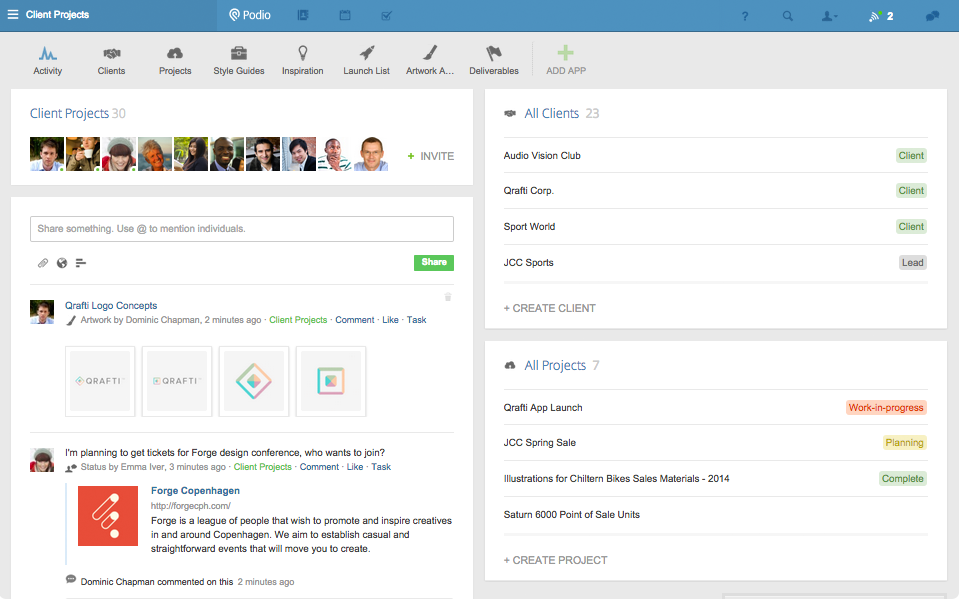
\includegraphics[scale=0.4]{Images/workspaces.png}
    \caption{Podio workspace}
    \label{fig:podio_workspace}
\end{figure}


\subsubsection{Bitrix24}
Bitrix24 is an online tool for project management, and collaboration for organizations. Bitrix24 focuses on social interactions in the organization and has features like tasks and project planning.\\
Bitrix24 has a full CRM system with a dashboard, a system for managing customer interactions and a system for sales. The CRM module makes it possible in the organization to have a clear overview of the customer and the sales and communication with the customer. The sales module has an access management system where the organization can control which employees have access to each customer and projects. The system also includes a mail system and a phone system, these systems make it possible to have all relevant contact logs and history directly associated with the project or the customer.\\
Bitrix24 has a project management system that integrates with the employees, the organization can define the roles of each employee and define access and tasks based on employee roles. The project management system has a integrated gantt chart to give a overview of the projects, tasks and time.\\
Bitrix24 has a system for employee time-management. Bitrix24 also supports apps, the apps can be added to the organizations Bitrix24\citep{website:Bitrixwhatis}. 

\subsubsection{WORK[etc]}
WORK[etc] is a web based CRM, Project management and collaboration system. WORK[etc] is made to be a complete solution, for businesses to help them manage their company.\\
The system has many features for both CRM, Project management and collaboration. The CRM module has features that allows, the company to create new clients in the system, where the clients information will be stored. The clients request can then be turned into a project, where employees will start to develop the product. The CRM module makes it possible for sales employees to administrate the process, as well as keep track of payments. The system can create a sales pipeline, for further helping the sales employees. \\
The project management module, has features for making new projects, where it is possible to connect clients to a specific project. The projects has different possibilities for making the development easier for the employees. The employees can discus on a open chat, and the project leaders can create new tasks. The module also contains functionality for making gantt charts, to visualize the progress of each active task. WORK[etc] also has a mobile platform, for both android and iPhone, and mail integration. \citep{website:WORK[etc]} 

\subsubsection{Summary}
Generally the different systems include functions such as project management, CRM and communication tools. These different functions go well together and it makes sense to integrate these into one homogeneous solution. 

Generally the systems looked at are all web-based. This is one of their strengths, as web-based applications have increased accessibility because they can be accessed through any browser. This is favorable for developers, as they only have to make a single version, that will work on any operating system that has a browser. It also makes the application easier to update, as you no longer need to push the update out to users, you just update the application on your own server. 
With a web app you can more easily sell your product as a subscription-based service\citep{website:subscription}. Selling your product via a subscription-based model, ensures that you have a steady income. It also cuts down on support and development times. Because every customer has access to the latest version of the software, the developer therefore only needs to consider the latest version of their product.

%Thus it would make sense for our project to also focus on these same aspects, as they are vital to every company. 

%• Hvilke ideer ser du i denne IT-anvendelse?
%• Virker ideerne gode? Hvorfor?
%• Vil ideerne kunne bruges i din sammenhæng. Hvorfor?
%• Kan ideerne tilpasses dit system? Hvordan?

% Beskriver de individuelle tjenester først, i summary forklares de gode ideer, og om hvorvidt
% de passer ind i vores system.


\subsection{Problem Definition}

%-- Gennem interviews, krav fra dorte er vi nået frem til at:
%-- ???? er de vigtigste funktioner at have med. Brugere sætter pris på web,
%-- brugervenlighed, at meget er samlet i et.

Through interviewing several startup companies, and from the requirements by Dorte Kjærgaard, the conclusion is that startup companies require a simple system that can help them manage their business more efficiently. A complicated set of systems with no integration with each other, only makes the process of running a company more complex, and takes away from the time that could be spent building the company. Most of the entrepreneurs interviewed requested an integrated system, with all their budgeting, CRM and project management in one place. What smaller companies need is one product that integrates the most important features, in a simple and easy to use package.
\\

\framebox{\parbox{\dimexpr\linewidth-2\fboxsep-2\fboxrule}{\itshape%
Startups need a simple system to help manage their business.

%How can the integration between management software for running a small company be done, and in such a way that makes the management process faster and easier?

How can business management software, that integrates the most essential features in a simple and easy to use way, be designed and developed?
}}

\subsection{System Definition}

From the information gathered, a system definition has been produced, that has have verified by using the FACTOR-criteria\citep{FACTORPage}. FACTOR-criteria is the name for a number of criteria that a system definition should fulfill.

Below is the system definition:

\framebox{\parbox{\dimexpr\linewidth-2\fboxsep-2\fboxrulex}{\itshape% 
A web application for running a newly started company. The application should be simple to use and can be accessed by a device running a modern browser and with access to to the internet. The application must have finance, CRM and project management modules. The finance module will give a overview on the budget and cash flow. The CRM module will be used for keeping information about the customers, such as their contact information, interactions and invoices. The project management module, will provide the ability to create multiple project workspaces, each with their own tasks and deadlines. Within each workspace you can create new tasks and assign users to complete them.The system will focus on businesses that deal in services and intangible goods.
}}\relax

As described in the system definition, the product should be an application that is really simple to use. It should provide an effective way for a entrepreneurs to manage their company.
If you divide the system definition up into the individual FACTOR-criteria, it would look like this:

\begin{itemize}
    \item \textbf{Functionality} The business owner can view and change finances, manage projects and the customer database. Employees can view the customer database and access and modify project data.
    \item \textbf{Application domain} Entrepreneurs and their employees.
    \item \textbf{Conditions} The system should make it simple for entrepreneurs to run their company and simple for employees to access tasks.
    \item \textbf{Technology} Any device running a modern browser and with access to to the internet.
    \item \textbf{Objects} Customers, companies, projects, financial data, users.
    \item \textbf{Responsibility} Providing administrative tools for entrepreneurs and tools for employees to collaborate on projects.
\end{itemize}


\begin{figure}[H]
    \centering
    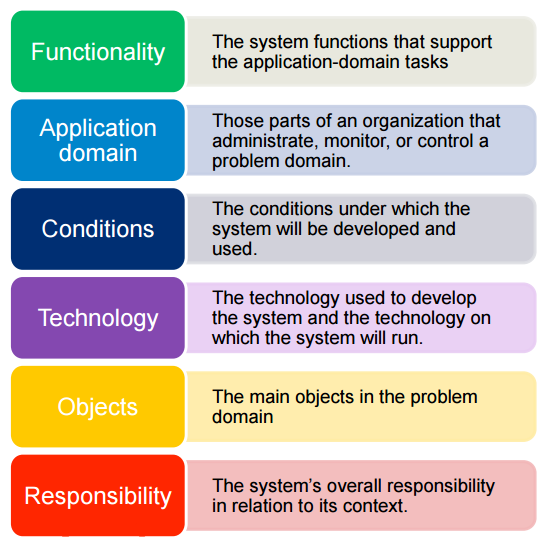
\includegraphics[scale=0.6]{Images/BATOFF.PNG}
    \caption{FACTOR-criteria, source: Jacob Nørbjerg, Systems Development Course: slide 3, 2015}
    \label{fig:FACTOR-criteria}
\end{figure}

\newpage

















